\documentclass[11pt,a4paper]{article}
\usepackage[margin=2.2cm]{geometry}
\usepackage{amsmath,amssymb,amsthm,mathtools,bm}
\usepackage{booktabs,array,longtable,enumitem}
\usepackage[dvipsnames]{xcolor}
\usepackage{tikz}
\usetikzlibrary{bayesnet,fit,positioning,backgrounds}
\usepackage[colorlinks=true,linkcolor=NavyBlue,citecolor=NavyBlue,urlcolor=NavyBlue]{hyperref}

\newcommand{\new}[1]{{\color{red}#1}}
\newcommand{\E}{\mathbb{E}}
\newcommand{\N}{\mathcal{N}}
\newcommand{\Bern}{\mathrm{Bern}}
\newcommand{\Betad}{\mathrm{Beta}}
\newcommand{\Gam}{\mathrm{Gamma}}
\newcommand{\logit}{\operatorname{logit}}
\newcommand{\diag}{\operatorname{diag}}
\newcommand{\ELBO}{\mathcal{L}}
\newcommand{\cfree}{\mathcal{C}_{\mathrm{free}}}
\newcommand{\wh}{\hat w}
% Results of notebook 04 (filled in after the run)
\newcommand{\RESCOHORT}{$\gamma$ AUC $0.873$ / $0.904$ (easy / hard) vs $0.864$ / $0.755$ for CohortFACTM with learned $\pi$; $\pi$ error $0.235$ / $0.105$ vs $0.291$ / $0.138$ (notebook 04).}
\newcommand{\RESFIT}{easy: mean $|$corr$|$ $0.921\to0.996$, pattern cells $0.90\to1.00$; hard: worst strong factor $0.878\to0.912$, pattern cells $0.95\to0.98$; multi-start reached the truth-start ELBO in every hard seed.}
\newcommand{\RESTABLES}{% generated by notebooks_sharedness/_results_tex.py -- do not edit by hand
\paragraph{Synthetic data (5 seeds per level).} Factor recovery is the Hungarian-matched $|\mathrm{corr}|$ with the true factors; ``strong'' excludes the deliberately weak factor of the hard level. Pattern recovery compares the called pattern ($a_{mk}\ge0.1$, or the frozen $\hat H$, or $\E h>0.5$) with $H$.
\begin{center}\footnotesize\setlength{\tabcolsep}{4pt}\begin{tabular}{@{}llrrrrr@{}}\toprule
level & arm & mean $|$corr$|$ & worst strong & worst (all) & cells correct & exact columns\\\midrule
easy & before (1 start, 400 sweeps) & 0.921 & 0.856 & 0.856 & 0.900 & 3.0/4\\
easy & multi-start, PCA start & 0.996 & 0.991 & 0.991 & 1.000 & 4.0/4\\
easy & multi-start, gCCA start & 0.996 & 0.991 & 0.991 & 1.000 & 4.0/4\\
easy & two-stage (final) & 0.995 & 0.989 & 0.989 & 1.000 & 4.0/4\\
easy & view switch, calibrated slab & 0.995 & 0.991 & 0.991 & 1.000 & 4.0/4\\
\midrule
hard & before (1 start, 400 sweeps) & 0.855 & 0.878 & 0.460 & 0.950 & 5.2/6\\
hard & multi-start, PCA start & 0.869 & 0.912 & 0.448 & 0.983 & 5.6/6\\
hard & multi-start, gCCA start & 0.843 & 0.911 & 0.288 & 0.975 & 5.4/6\\
hard & two-stage (final) & 0.842 & 0.910 & 0.285 & 0.975 & 5.4/6\\
hard & view switch, calibrated slab & 0.845 & 0.912 & 0.288 & 0.975 & 5.4/6\\
\bottomrule\end{tabular}\end{center}
The calibrated view switch has 50.0\% / 47.5\% of switches on (truth $50\%$) and switch AUC 1.00 / 0.99 (easy / hard). Refinement flipped 0.0 cells on average.
\paragraph{Cohort prior (3 seeds $\times$ true rates $0.1,0.3,0.6$, $C=6$).} $\gamma$ AUC: ranking of $\E\gamma$ against the true switches; null/alt: mean $\E\gamma$ where the truth is $0$/$1$.
\begin{center}\footnotesize\setlength{\tabcolsep}{4pt}\begin{tabular}{@{}llrrrr@{}}\toprule
level & arm & $|\E\pi-\pi^\ast|$ & $\gamma$ AUC & null $\E\gamma$ & alt $\E\gamma$\\\midrule
easy & CohortFACTM, $\pi=0.5$ fixed & 0.208 & 0.841 & 0.458 & 0.858\\
easy & CohortFACTM, $\pi$ learned & 0.291 & 0.864 & 0.586 & 0.957\\
easy & \textbf{paired, $\pi$ learned (final)} & 0.235 & 0.873 & 0.487 & 0.931\\
easy & scale-free paired (V1) & 0.337 & 0.869 & 0.630 & 0.972\\
easy & reference cohort (V2) & 0.163 & 0.619 & 0.650 & 0.821\\
\midrule
hard & CohortFACTM, $\pi=0.5$ fixed & 0.244 & 0.883 & 0.148 & 0.754\\
hard & CohortFACTM, $\pi$ learned & 0.138 & 0.755 & 0.085 & 0.531\\
hard & \textbf{paired, $\pi$ learned (final)} & 0.105 & 0.904 & 0.332 & 0.893\\
hard & scale-free paired (V1) & 0.107 & 0.904 & 0.355 & 0.901\\
hard & reference cohort (V2) & 0.121 & 0.642 & 0.456 & 0.652\\
\bottomrule\end{tabular}\end{center}
The reference arm is scored against shifts relative to the reference cohort (different truth).
\paragraph{Real data (3 seeds; 4 starts).} Stability across seeds: correlation of the activity matrices and Hungarian-matched factor correlation (mean, and mean of the worst factor).
\begin{center}\footnotesize\setlength{\tabcolsep}{4pt}\begin{tabular}{@{}llrrr@{}}\toprule
data & arm & activity corr & mean factor match & worst factor match\\\midrule
COVID (M=2) & before & 0.724 & 0.738 & 0.572\\
COVID (M=2) & multistart & 0.962 & 0.762 & 0.582\\
COVID (M=2) & two-stage & 0.977 & 0.862 & 0.624\\
four-view (M=4) & before & 0.898 & 0.785 & 0.580\\
four-view (M=4) & multistart & 1.000 & 0.999 & 0.999\\
four-view (M=4) & two-stage & 1.000 & 1.000 & 1.000\\
\bottomrule\end{tabular}\end{center}
\begin{center}\footnotesize\setlength{\tabcolsep}{4pt}\begin{tabular}{@{}llrrr@{}}\toprule
data & cohort prior & $\E\pi$ & switches on ($>0.9$) & switches off ($<0.1$)\\\midrule
COVID (M=2) & CohortFACTM, $\pi$ learned & 0.92 $\pm$ 0.06 & 100\% & 0\%\\
COVID (M=2) & \textbf{paired, $\pi$ learned (final)} & 0.52 $\pm$ 0.12 & 40\% & 47\%\\
COVID (M=2) & scale-free paired (V1) & 0.60 $\pm$ 0.12 & 47\% & 7\%\\
four-view (M=4) & CohortFACTM, $\pi$ learned & 0.97 $\pm$ 0.03 & 100\% & 0\%\\
four-view (M=4) & \textbf{paired, $\pi$ learned (final)} & 0.88 $\pm$ 0.05 & 83\% & 0\%\\
four-view (M=4) & scale-free paired (V1) & 0.90 $\pm$ 0.05 & 83\% & 0\%\\
\bottomrule\end{tabular}\end{center}
}

\newtheorem{proposition}{Proposition}
\newtheorem{lemma}{Lemma}
\newtheorem{conjecture}{Conjecture}
\theoremstyle{definition}
\newtheorem{definition}{Definition}
\theoremstyle{remark}
\newtheorem*{remark}{Remark}

\title{SP-CohortFACTM: a shared/private extension of CohortFACTM\\[2pt]
\large Model, variational family, updates, fitting procedure, results and open proofs}
\author{Karol Jurasz \quad (branch \texttt{first\_ideas\_karol})}
\date{19 October 2026}

\begin{document}
\maketitle

\noindent\textbf{How to read.} Everything marked \new{in red} is new or changed with respect to CohortFACTM as
implemented in the repository before this branch; black terms are unchanged. All names introduced here are defined in
the glossary (Section~\ref{sec:glossary}), all symbols in Table~\ref{tab:notation}. Implementation: package
\texttt{sharedness/} and the corrected \texttt{src/w\_priors/ARD\_SS.py}. Every update below is tested for ELBO
monotonicity and stationarity (\texttt{tests/test\_sharedness\_priors.py}, 26 tests), and the formulas were checked
against the code by an independent reviewer.

\tableofcontents

%======================================================================
\section{Glossary}\label{sec:glossary}
%======================================================================
\begin{description}[leftmargin=0pt,itemsep=3pt]
\item[View, modality.] A block $Y^{(m)}\in\mathbb R^{N\times D_m}$ of features measured on the same $N$ samples.
  Views partition the \emph{features}; cohorts partition the \emph{samples}.
\item[View pattern $H$.] $H\in\{0,1\}^{M\times K}$ with $H_{mk}=1$ iff view $m$ uses factor $k$, i.e.\ the loading column
  $w^{(m)}_{\cdot k}$ may be non-zero. Factor $k$ is \emph{shared} if $H_{\cdot k}=\mathbf 1$, \emph{partially shared} if
  $1<\sum_mH_{mk}<M$, \emph{private} to view $m$ if $H_{\cdot k}=e_m$, \emph{inactive} if $H_{\cdot k}=\mathbf 0$.
\item[Switch.] A Bernoulli latent variable that turns a component on or off: the \emph{element switch} $s^{(m)}_{dk}$
  (is loading $w^{(m)}_{dk}$ non-zero?), the \emph{cohort switch} $\gamma_{ck}$ (does cohort $c$ have its own mean on
  factor $k$?), and the optional \emph{view switch} $h_{mk}$ (does view $m$ use factor $k$?).
\item[Spike and slab.] ``Switch on: draw from a continuous \emph{slab}; switch off: exactly $0$ (the \emph{spike})''.
\item[Paired factorisation.] A variational family that keeps a switch and the quantity it gates together,
  $q(\text{switch},\text{value})=q(\text{switch})\,q(\text{value}\mid\text{switch})$, instead of the fully factorised
  $q(\text{switch})\,q(\text{value})$. \emph{Paired cohort prior}: CohortFACTM's cohort prior fitted with the paired family
  for $(\gamma_{ck},\delta_{ck})$.
\item[Occam term.] The part of a switch's log-odds that penalises switching on even when the data are fitted equally
  well: the log-ratio of prior to posterior volume of the gated parameter, e.g.\ $-\tfrac12\log(1+\tau n_c/\lambda)$.
\item[Variance share, activity.] $r_{mk}=\|\E z_{\cdot k}\,\E w^{(m)\top}_{\cdot k}\|_F^2/\|Y^{(m)}\|_F^2$, the fraction of view $m$'s
  variance carried by factor $k$; activity $a_{mk}=r_{mk}/\max_{m'}r_{m'k}\in[0,1]$.
\item[Learned vs frozen (prescribed) pattern.] Learned: $H$ (or $h$) is updated by CAVI. Frozen: $H$ is fixed during the
  fit and masked columns are exact zeros.
\item[Two-stage fit.] Stage 1 fits without a view pattern; stage 2 freezes $\hat H_{mk}=\mathbb 1\{a_{mk}\ge t\}$ read off
  stage 1 and refits; a refinement step flips borderline cells if that raises the ELBO.
\item[Multi-start.] Several fits from different initial rotations; the fit with the highest ELBO is kept.
\item[gCCA start.] Initialisation by generalised canonical correlation analysis (MAXVAR), which separates directions
  shared by several views from view-specific ones (Section~\ref{sec:init}).
\item[Scale-free shift prior] (evaluated variant). $\delta_{ck}\mid\tau_{ck}\sim\N(0,(\kappa\tau_{ck})^{-1})$: the shift in units of
  the cohort's own standard deviation (Section~\ref{sec:variants}).
\item[Reference cohort] (evaluated variant). A cohort $c_0$ whose switch is fixed off; the data are centred on $c_0$ so
  that shifts are relative to it (Section~\ref{sec:variants}).
\item[SP-CohortFACTM.] The model of this document: CohortFACTM with the paired cohort prior and a learned global
  $\pi$, the corrected element spike-and-slab on the loadings, and a frozen view pattern $H$, fitted by the two-stage
  multi-start procedure.
\end{description}

%======================================================================
\section{Notation}
%======================================================================
\begin{table}[h]\centering\footnotesize
\caption{Symbols. Row convention: $y_n^{(m)}=W^{(m)}z_n+\varepsilon$, $Z\in\mathbb R^{N\times K}$, $W^{(m)}\in\mathbb R^{D_m\times K}$.}
\label{tab:notation}
\begin{tabular}{@{}ll@{}}\toprule
$n=1..N$; $m=1..M$; $d=1..D_m$; $k=1..K$ & samples; views; features of view $m$; factors\\
$c=1..C$, $c(n)$, $n_c=|\{n:c(n)=c\}|$ & cohorts, cohort of sample $n$, cohort size\\
$y^{(m)}_{nd}$ & data (centred per feature)\\
$z_{nk}$ & factor score\\
$w^{(m)}_{dk}=H_{mk}\,s^{(m)}_{dk}\,\wh^{(m)}_{dk}$ & loading = view gate $\times$ element switch $\times$ slab value\\
$\alpha_{mk}$, $\theta_{mk}$ & ARD precision and element inclusion rate of column $k$ in view $m$\\
$\tau_{md}$ & noise precision of feature $d$ in view $m$\\
$\gamma_{ck}$, $\delta_{ck}$, $\tau_{ck}$, $\lambda_k$ & cohort switch, cohort shift, within-cohort precision, shift precision\\
$\pi$ & cohort switch rate (learned)\\
$S_{ck}=\sum_{n\in c}m_{nk}$, $Q_{ck}=\sum_{n\in c}(m^2_{nk}+\varsigma^2_{nk})$ & cohort sums of factor moments\\
$\psi$, $\sigma(u)=1/(1+e^{-u})$, $\langle\cdot\rangle$ & digamma, logistic, expectation under $q$\\
\bottomrule\end{tabular}
\end{table}

%======================================================================
\section{The model}
%======================================================================
\subsection{Generative model}
\begin{align}
y^{(m)}_{nd}\mid z,w,\tau &\sim \N\Big(\textstyle\sum_{k} w^{(m)}_{dk}z_{nk},\ \tau_{md}^{-1}\Big), &\tau_{md}&\sim\Gam(a_0,b_0),\label{eq:lik}\\
w^{(m)}_{dk} &= \new{H_{mk}}\, s^{(m)}_{dk}\,\wh^{(m)}_{dk}, &\new{H}&\ \new{\text{fixed constant, chosen between fits (Rem.~\ref{rem:H})}},\label{eq:w}\\
\wh^{(m)}_{dk}\mid\alpha_{mk}&\sim\N(0,\alpha_{mk}^{-1}), &\alpha_{mk}&\sim\Gam(a_\alpha,b_\alpha),\\
s^{(m)}_{dk}\mid\theta_{mk}&\sim\Bern(\theta_{mk}), &\theta_{mk}&\sim\Betad(a_\theta,b_\theta),\\
z_{nk}\mid c(n)=c &\sim \N\big(\gamma_{ck}\delta_{ck},\ \tau_{ck}^{-1}\big), &\tau_{ck}&\sim\Gam(a_\tau,b_\tau),\label{eq:z}\\
\delta_{ck}\mid\lambda_k &\sim \N\big(0,\ \lambda_k^{-1}\big), &\lambda_k&\sim\Gam(a_\lambda,b_\lambda),\label{eq:delta}\\
\gamma_{ck}\mid\pi &\sim\Bern(\pi), &\new{\pi}&\new{\ \sim\Betad(a_\pi,b_\pi)}\quad(\text{CohortFACTM: }\pi\text{ fixed}).\label{eq:gamma}
\end{align}
Hyperparameters: $a_0=b_0=10^{-3}$, $a_\alpha=b_\alpha=10^{-14}$, $a_\theta=b_\theta=1$, $a_\tau=b_\tau=1$, $a_\lambda=b_\lambda=1$,
$a_\pi=b_\pi=1$. On data without cohort structure the cohort prior is replaced by $z_{nk}\sim\N(0,1)$. Structured (CTM)
views of FACTM enter unchanged through their usual precision and linear term on $z_{nk}$; they were not used in the
experiments and are omitted below. The model is unchanged from CohortFACTM except for $H$ and $\pi$; what changes most is
the \emph{variational family} (Section~\ref{sec:q}) and the \emph{fitting procedure} (Section~\ref{sec:fit}).

\begin{figure}[h]\centering
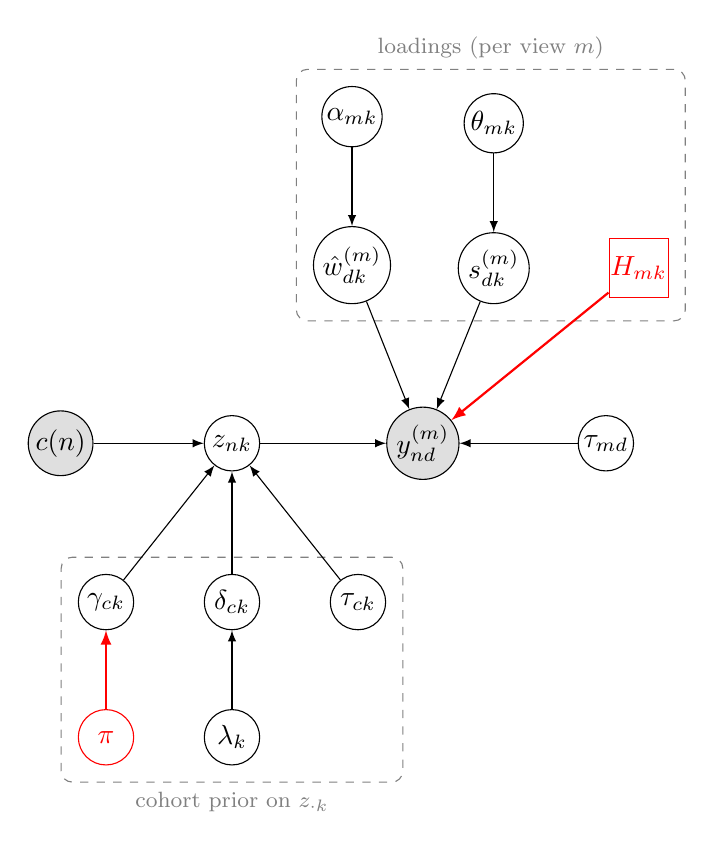
\begin{tikzpicture}[node distance=1.25cm, >=latex]
  \node[obs] (y) {$y^{(m)}_{nd}$};
  \node[latent, left=1.6cm of y] (z) {$z_{nk}$};
  \node[latent, right=1.5cm of y] (tn) {$\tau_{md}$};
  \node[latent, above=1.3cm of y, xshift=-0.9cm] (wh) {$\wh^{(m)}_{dk}$};
  \node[latent, above=1.3cm of y, xshift=0.9cm] (s) {$s^{(m)}_{dk}$};
  \node[latent, above=of wh] (al) {$\alpha_{mk}$};
  \node[latent, above=of s] (th) {$\theta_{mk}$};
  \node[const, right=1.0cm of s, draw=red, text=red, rectangle, minimum size=0.75cm] (H) {$H_{mk}$};
  \node[latent, below=1.3cm of z, xshift=-1.6cm] (g) {$\gamma_{ck}$};
  \node[latent, below=1.3cm of z] (dl) {$\delta_{ck}$};
  \node[latent, below=1.3cm of z, xshift=1.6cm] (tc) {$\tau_{ck}$};
  \node[latent, below=of g, draw=red, text=red] (pi) {$\pi$};
  \node[latent, below=of dl] (lam) {$\lambda_k$};
  \node[obs, left=1.4cm of z] (c) {$c(n)$};
  \edge {z,wh,s,tn} {y};
  \draw[->, red, thick] (H) -- (y);
  \edge {al} {wh};
  \edge {th} {s};
  \edge {g,dl,tc,c} {z};
  \edge {lam} {dl};
  \draw[->, red, thick] (pi) -- (g);
  \begin{scope}[on background layer]
    \node[draw=gray, dashed, rounded corners, fit=(wh)(s)(al)(th)(H), inner sep=6pt,
          label={[gray]above:loadings (per view $m$)}] {};
    \node[draw=gray, dashed, rounded corners, fit=(g)(dl)(tc)(pi)(lam), inner sep=6pt,
          label={[gray]below:cohort prior on $z_{\cdot k}$}] {};
  \end{scope}
\end{tikzpicture}
\caption{SP-CohortFACTM. Circles: latent; shaded: observed; boxed: fixed. \new{Red}: new relative to CohortFACTM ---
the frozen view pattern $H$ gating whole loading columns, and the learned switch rate $\pi$. The paired variational
family (not visible in a graphical model) is the third change.}
\label{fig:model}
\end{figure}

\subsection{What the model assumes}
\begin{enumerate}[itemsep=2pt]
\item One score vector $z_n$ drives all views (the FACTM backbone).
\item \new{View pattern.} Factor $k$ may be absent from view $m$ as a whole: if $H_{mk}=0$ the column $w^{(m)}_{\cdot k}$ is
  exactly zero. Within a used column individual loadings may be zero (element sparsity).
\item Cohort structure acts on the factors: cohort $c$ either shares the common mean of factor $k$ ($\gamma_{ck}=0$) or has
  its own shift $\delta_{ck}$; each cohort has its own spread $\tau_{ck}^{-1}$. Because the data are centred on the grand mean,
  ``own shift'' means ``differs from the grand mean''.
\item \new{The probability that a cohort shifts is learned} from all $CK$ cohort switches.
\end{enumerate}

%======================================================================
\section{Variational family}\label{sec:q}
%======================================================================
\begin{equation}\label{eq:q}
\begin{split}
q={}&\prod_{n,k}q(z_{nk})\prod_{m,k}\Big[q(\alpha_{mk})q(\theta_{mk})\prod_d \new{q(s^{(m)}_{dk})\,q(\wh^{(m)}_{dk}\mid s^{(m)}_{dk})}\Big]\prod_{m,d}q(\tau_{md})\\
&\times\prod_{k}q(\lambda_k)\prod_{c,k}\Big[q(\tau_{ck})\,\new{q(\gamma_{ck})\,q(\delta_{ck}\mid\gamma_{ck})}\Big]\,\new{q(\pi)}
\end{split}
\end{equation}
with
\begin{align*}
q(z_{nk})&=\N(m_{nk},\varsigma^2_{nk}), & q(\tau_{md})&=\Gam(a^\tau_{md},b^\tau_{md}),\\
q(\alpha_{mk})&=\Gam(a^\alpha_{mk},b^\alpha_{mk}), & q(\theta_{mk})&=\Betad(a^\theta_{mk},b^\theta_{mk}),\\
q(s^{(m)}_{dk})&=\Bern(g^{(m)}_{dk}), & q(\wh^{(m)}_{dk}\mid s=1)&=\N(\mu_{dk},\sigma^2_{dk}),\quad \new{q(\wh^{(m)}_{dk}\mid s=0)=\N(0,v^{w}_{0,mk})},\\
q(\tau_{ck})&=\Gam(a_{ck},b_{ck}), & q(\gamma_{ck})&=\Bern(\rho_{ck}),\\
q(\delta_{ck}\mid\gamma=1)&=\N(\mu^\delta_{ck},v^\delta_{ck}), & \new{q(\delta_{ck}\mid\gamma=0)}&\new{=\N(0,v^\delta_{0,k})},\\
q(\lambda_k)&=\Gam(a^\lambda_k,b^\lambda_k), & \new{q(\pi)}&\new{=\Betad(a^\pi,b^\pi)}.
\end{align*}
For a masked column ($H_{mk}=0$) the factors $s_{\cdot k},\wh_{\cdot k},\theta_{mk},\alpha_{mk}$ are absent: the masked model has
$w^{(m)}_{\cdot k}\equiv0$. (In the code: masked $\logit g=-50$, masked $q(\theta)$ held at its prior, and the masked terms
removed from the ELBO.)

\begin{remark}[Why $H$ has no prior and no $q$]\label{rem:H}
$H$ is \new{not a latent variable}. It is a \emph{fixed structural constant} of the fitted model, like the number of
factors $K$ or the assignment of features to views: the likelihood is conditioned on $H$, not generative in it. Hence
$H$ has no prior $p(H)$ in~\eqref{eq:q}, no variational factor $q(H)$, and no CAVI update --- it never changes during a
fit. It is instead chosen \emph{between} fits, by the two-stage, evidence-based procedure of Section~\ref{sec:fit}:
stage~1 fits with $H\equiv1$, $\hat H_{mk}=\mathbb 1\{a_{mk}\ge t\}$ is read off that fit (a point estimate, not a
distribution), stage~2 freezes $H=\hat H$, and the refinement step compares neighbouring patterns by their stage-2
ELBO (discrete model selection, as in SLIDE). This is deliberate: giving the view pattern a $\Bern(\pi_h)$ prior and a
$q(h_{mk})$ updated inside CAVI --- the \emph{view switch} (variant V3, Section~\ref{sec:variants}) --- is a valid model,
but then the pattern is \emph{learned}, not frozen, and the model can always switch a masked column back on at an
$O(MK)$ prior cost, which destroys the likelihood-level identification of the split (Conjecture~\ref{conj:growth},
Lemma~\ref{lem:hid}). The three \emph{switches} that do have a prior and a $q$ --- $s^{(m)}_{dk}$, $\gamma_{ck}$, and (if
used) $h_{mk}$ --- are summarised against $H$ in Table~\ref{tab:switches}.
\end{remark}

\begin{table}[h]\centering\footnotesize
\caption{The on/off structures in the model: which are latent (inferred inside CAVI) and which are fixed.}
\label{tab:switches}
\begin{tabular}{@{}lllll@{}}\toprule
object & gates & latent? & prior & $q$\\\midrule
$s^{(m)}_{dk}$ element switch & one loading $w^{(m)}_{dk}$ & yes & $\Bern(\theta_{mk})$ & $\Bern(g^{(m)}_{dk})$\\
$\gamma_{ck}$ cohort switch & one cohort mean $\delta_{ck}$ & yes & $\Bern(\pi)$ & $\Bern(\rho_{ck})$\\
$h_{mk}$ view switch (V3, not adopted) & one loading column $w^{(m)}_{\cdot k}$ & yes & $\Bern(\pi_h)$ & $\Bern(\E h_{mk})$\\
\new{$H_{mk}$ frozen view pattern (adopted)} & \new{one loading column $w^{(m)}_{\cdot k}$} & \new{no (fixed)} & \new{---} & \new{---}\\
\bottomrule\end{tabular}
\end{table}

\begin{remark}[What changed in $q$, and why]
CohortFACTM uses $q(\gamma_{ck})\,q(\delta_{ck})$. Then, with $q(\delta)$ at its optimum, the switch's update carries no
$\log n_c$ Occam term (Lemma~\ref{lem:noocc}), so switches without real evidence are not pushed off and a learned $\pi$
drifts upwards. The paired family restores the term. The repository's element spike-and-slab (\texttt{ARD\_SS})
intended the paired form for $(s,\wh)$ but its update and ELBO did not match each other; both now follow the paired
family.
\end{remark}

%======================================================================
\section{The ELBO}
%======================================================================
$\ELBO(q)=\E_q[\log p(Y,\Theta)]-\E_q[\log q(\Theta)]=\sum_{j=1}^{8}\ELBO_j$. Moments:
$\E w^{(m)}_{dk}=H_{mk}g\mu$, $\E[(w^{(m)}_{dk})^2]=H_{mk}g(\sigma^2+\mu^2)$, $\E[\wh^2]=g(\sigma^2+\mu^2)+(1-g)v_0^w$,
$\E[\gamma\delta]=\rho\mu^\delta$, $\E[\gamma\delta^2]=\rho(v^\delta+\mu^{\delta2})$, $\E[\delta^2]=\rho(v^\delta+\mu^{\delta2})+(1-\rho)v_0^\delta$.

\paragraph{$\ELBO_1$: likelihood.}
$\displaystyle\ELBO_1=\sum_{m,n,d}\Big[\tfrac12\big(\langle\log\tau_{md}\rangle-\log2\pi\big)-\tfrac12\langle\tau_{md}\rangle\,
\E\Big(y^{(m)}_{nd}-\textstyle\sum_k w^{(m)}_{dk}z_{nk}\Big)^2\Big]$, where
\[
\E\Big(y-\textstyle\sum_k w_kz_k\Big)^2=\Big(y-\textstyle\sum_k\E w_k\,m_k\Big)^2+\textstyle\sum_k\big(\E[w_k^2](m_k^2+\varsigma_k^2)-(\E w_k)^2m_k^2\big).
\]

\paragraph{$\ELBO_2$: noise.} $\sum_{m,d}\big(\E\log\Gam(\tau_{md}\mid a_0,b_0)+\mathbb H[q(\tau_{md})]\big)$, with
$\mathbb H[\Gam(a,b)]=a-\log b+\log\Gamma(a)+(1-a)\psi(a)$.

\paragraph{$\ELBO_3$: loadings.} For a used column ($H_{mk}=1$), per feature $d$:
\begin{align*}
&\underbrace{g\big[\tfrac12\langle\log\alpha\rangle-\tfrac12\langle\alpha\rangle(\sigma^2+\mu^2)+\tfrac12\log\sigma^2+\tfrac12\big]}_{\text{slab: }\E\log p(\wh\mid\alpha)+\mathbb H[q(\wh\mid s=1)]}
+\underbrace{\new{(1-g)\big[\tfrac12\langle\log\alpha\rangle-\tfrac12\langle\alpha\rangle v_0^w+\tfrac12\log v_0^w+\tfrac12\big]}}_{\text{spike branch}}\\
&\qquad+g\langle\log\theta\rangle+(1-g)\langle\log(1-\theta)\rangle-g\log g-(1-g)\log(1-g).
\end{align*}
\new{A masked column contributes nothing.} (Keeping its $s,\theta,\alpha$ with $s\equiv0$ would add about $-\log(D_m+1)$
nats per masked cell and bias comparisons of patterns against masking.) The previous \texttt{ARD\_SS} ELBO used
$\E[1/\alpha]$ in the spike branch and dropped the slab's $+\tfrac12$, so it did not match its own update.

\paragraph{$\ELBO_4$: ARD precisions and inclusion rates} of used columns:
$\sum_{m,k:H_{mk}=1}\big(\E\log\Gam(\alpha_{mk})+\mathbb H[q(\alpha_{mk})]+\E\log\Betad(\theta_{mk})+\mathbb H[q(\theta_{mk})]\big)$.

\paragraph{$\ELBO_5$: factors.} For each $(c,k)$:
$\tfrac12n_c\big(\langle\log\tau_{ck}\rangle-\log2\pi\big)-\tfrac12\langle\tau_{ck}\rangle\big(Q_{ck}-2\rho\mu^\delta S_{ck}+n_c\rho(v^\delta+\mu^{\delta2})\big)
+\tfrac12\sum_{n\in c}\big(1+\log2\pi+\log\varsigma^2_{nk}\big)$.

\paragraph{$\ELBO_6$: cohort shifts.} Per $(c,k)$ ($2\pi$ terms cancel):
\[
\tfrac12\langle\log\lambda_k\rangle-\tfrac12\langle\lambda_k\rangle\big[\rho(v^\delta+\mu^{\delta2})\new{+(1-\rho)v_0^\delta}\big]
+\tfrac12\big[\rho\log v^\delta\new{+(1-\rho)\log v^\delta_0}\big]+\tfrac12.
\]
(CohortFACTM: $\tfrac12\langle\log\lambda_k\rangle-\tfrac12\langle\lambda_k\rangle\E\delta^2+\tfrac12\log v^\delta+\tfrac12$ with a single $q(\delta)$.)

\paragraph{$\ELBO_7$: cohort switches.}
$\sum_{c,k}\big[\rho_{ck}\new{\langle\log\pi\rangle}+(1-\rho_{ck})\new{\langle\log(1-\pi)\rangle}-\rho_{ck}\log\rho_{ck}-(1-\rho_{ck})\log(1-\rho_{ck})\big]$
(CohortFACTM: $\log\pi$, $\log(1-\pi)$ with fixed $\pi$).

\paragraph{$\ELBO_8$: precisions \new{and $\pi$}.}
$\sum_{c,k}\big(\E\log\Gam(\tau_{ck})+\mathbb H[q(\tau_{ck})]\big)+\sum_k\big(\E\log\Gam(\lambda_k)+\mathbb H[q(\lambda_k)]\big)
+\new{\E\log\Betad(\pi\mid a_\pi,b_\pi)+\mathbb H[q(\pi)]}$, with
$\mathbb H[\Betad(a,b)]=\log B(a,b)-(a-1)\psi(a)-(b-1)\psi(b)+(a+b-2)\psi(a+b)$.

\subsection{Occam penalties and the other weights}\label{sec:occam}
Optimising the gated parameter out of each paired block splits the switch's log-odds into evidence and an Occam term:
\begin{align}
\text{element switch:}\quad&\underbrace{\tfrac12\log\frac{\langle\alpha_{mk}\rangle}{\Lambda_{dk}}}_{\text{Occam}}+\underbrace{\frac{\nu_{dk}^2}{2\Lambda_{dk}}}_{\text{evidence}},
  \qquad \tfrac12\log\frac{\langle\alpha_{mk}\rangle}{\Lambda_{dk}}=-\tfrac12\log\Big(1+\frac{\sum_n\langle\tau_{md}\rangle\langle z_{nk}^2\rangle}{\langle\alpha_{mk}\rangle}\Big),\\
\text{cohort switch:}\quad&\underbrace{\new{-\tfrac12\log\Big(1+\frac{\langle\tau_{ck}\rangle n_c}{\langle\lambda_k\rangle}\Big)}}_{\text{Occam}}
  +\underbrace{\frac{\langle\tau_{ck}\rangle^2S_{ck}^2}{2(\langle\lambda_k\rangle+\langle\tau_{ck}\rangle n_c)}}_{\text{evidence}},\\
\text{view pattern (frozen):}\quad&\text{no switch; } H_{mk}=0 \text{ is a hard constraint.}\notag
\end{align}
No tempering weights are used: every ELBO term has weight $1$. Tuning constants: the pattern threshold $t=0.1$, the
refinement band $[0.05,0.3)$, the gCCA threshold $1.5$ and the number of starts.

\begin{lemma}[CohortFACTM's switch has no $\log n$ Occam term]\label{lem:noocc}
Under $q(\gamma_{ck})q(\delta_{ck})$, with $q(\delta_{ck})$ at its optimum and $\langle\lambda_k\rangle\ll\rho_{ck}\langle\tau_{ck}\rangle n_c$, the
stationarity condition for $\rho=\rho_{ck}$ is
\[\logit\rho=\logit\pi+\tfrac12\langle\tau_{ck}\rangle S_{ck}^2/n_c-\frac{1}{2\rho}+o(1).\]
Hence the switch carries no penalty growing like $\tfrac12\log n_c$, only the bounded $-1/(2\rho)$. Since
$f(\rho)=\logit\rho+1/(2\rho)$ has minimum $f(1/3)=1.5-\log2\approx0.807$, an interior solution exists iff
$\logit\pi+\tfrac12\langle\tau\rangle S^2/n\ge0.807$. Under the null ($\langle\tau\rangle S^2/n=X\sim\chi^2_1$): at $\pi=0.5$ this holds for
about $20\%$ of null cohorts (the rest go to $\rho\approx0$); for $\pi\ge0.7$ it always holds and $\rho$ settles just below
$\pi$ (e.g.\ $0.88$ at $\pi=0.9$). A learned $\pi$ therefore reinforces itself once it is large.
\end{lemma}
\begin{proof}
CohortFACTM's update is $\logit\rho=\logit\pi-\tfrac12\langle\tau\rangle(n\,\E\delta^2-2\,\E\delta\,S)$ with $q(\delta)=\N(\mu,v)$,
$\mu=\langle\tau\rangle\rho S/P$, $v=1/P$, $P=\langle\lambda\rangle+\langle\tau\rangle\rho n$. If $\lambda\ll\tau\rho n$: $\mu\to S/n$, $v\to1/(\tau\rho n)$, so
$n(v+\mu^2)-2\mu S\to\frac{1}{\tau\rho}-\frac{S^2}{n}$ and $-\tfrac12\tau\big(n(v+\mu^2)-2\mu S\big)\to-\frac1{2\rho}+\tfrac12\tau S^2/n$. For the
threshold, $f'(\rho)=\frac{1}{\rho(1-\rho)}-\frac1{2\rho^2}=0\iff\rho=1/3$. \qedhere
\end{proof}
\begin{remark}
The profiled ELBO ($q(\delta)$ optimised for each $\rho$) still contains the full Occam term between $\rho=0$ and $\rho=1$,
but it sits in a barrier near $\rho\approx0$ that coordinate ascent under $q(\gamma)q(\delta)$ does not cross. The paired
family removes the barrier by optimising $q(\delta\mid\gamma)$ separately in each branch.
\end{remark}

%======================================================================
\section{Coordinate updates}
%======================================================================
Each update is the exact maximiser of $\ELBO$ in its block given all others (conjugate exponential-family updates;
Proposition~\ref{prop:cavi}). Residual without factor $k$: $r^{(-k)}_{nd}=y^{(m)}_{nd}-\sum_{k'\neq k}\E w^{(m)}_{dk'}m_{nk'}$.

\paragraph{Factors $q(z_{nk})$} (unchanged):
\[
\varsigma^{-2}_{nk}=\langle\tau_{c(n)k}\rangle+\sum_{m,d}\langle\tau_{md}\rangle\E[(w^{(m)}_{dk})^2],\qquad
m_{nk}=\varsigma^2_{nk}\Big(\langle\tau_{c(n)k}\rangle\rho_{c(n)k}\mu^\delta_{c(n)k}+\sum_{m,d}\langle\tau_{md}\rangle\E w^{(m)}_{dk}\,r^{(-k)}_{nd}\Big).
\]

\paragraph{Cohort block for factor $k$} (\new{paired}; replaces CohortFACTM's $\delta$ and $\gamma$ updates). For every cohort $c$:
\begin{align*}
v^\delta_{ck}&=\frac{1}{\langle\lambda_k\rangle+\langle\tau_{ck}\rangle n_c},\qquad \mu^\delta_{ck}=v^\delta_{ck}\langle\tau_{ck}\rangle S_{ck},\qquad
\new{v^\delta_{0,k}=1/\langle\lambda_k\rangle},\\
\logit\rho_{ck}&=\new{\langle\log\pi\rangle-\langle\log(1-\pi)\rangle}+\new{\tfrac12\log\frac{\langle\lambda_k\rangle}{\langle\lambda_k\rangle+\langle\tau_{ck}\rangle n_c}}+\frac{\langle\tau_{ck}\rangle^2S^2_{ck}}{2(\langle\lambda_k\rangle+\langle\tau_{ck}\rangle n_c)},\\
a_{ck}&=a_\tau+\tfrac{n_c}{2},\qquad b_{ck}=b_\tau+\tfrac12\big(Q_{ck}-2\rho_{ck}\mu^\delta_{ck}S_{ck}+n_c\rho_{ck}(v^\delta_{ck}+\mu^{\delta2}_{ck})\big),\\
a^\lambda_k&=a_\lambda+\tfrac C2,\qquad b^\lambda_k=b_\lambda+\tfrac12\textstyle\sum_c\big[\rho_{ck}(v^\delta_{ck}+\mu^{\delta2}_{ck})\new{+(1-\rho_{ck})v^\delta_{0,k}}\big],\\
\new{a^\pi}&\new{=a_\pi+\textstyle\sum_{c,k}\rho_{ck},\qquad b^\pi=b_\pi+CK-\sum_{c,k}\rho_{ck}}.
\end{align*}
(CohortFACTM: $v^\delta=1/(\langle\lambda\rangle+\langle\tau\rangle\rho n)$, $\mu^\delta=v^\delta\langle\tau\rangle\rho S$, and
$\logit\rho=\logit\pi-\tfrac12\langle\tau\rangle(n\E\delta^2-2\E\delta\,S)$, i.e.\ $q(\delta)$ shared by both branches.)

\paragraph{Loadings of a used column ($H_{mk}=1$).} With $\Lambda_{dk}=\sum_n\langle\tau_{md}\rangle(m_{nk}^2+\varsigma^2_{nk})+\langle\alpha_{mk}\rangle$ and
$\nu_{dk}=\sum_n\langle\tau_{md}\rangle m_{nk}r^{(-k)}_{nd}$:
\begin{gather*}
\mu_{dk}=\nu_{dk}/\Lambda_{dk},\qquad \sigma^2_{dk}=1/\Lambda_{dk},\qquad \new{v^w_{0,mk}=1/\langle\alpha_{mk}\rangle},\\
\logit g_{dk}=\psi(a^\theta)-\psi(b^\theta)+\tfrac12\log\langle\alpha_{mk}\rangle\new{\,-\,}\tfrac12\log\Lambda_{dk}+\frac{\nu_{dk}^2}{2\Lambda_{dk}}.
\end{gather*}
(Previously $+\tfrac12\log\Lambda_{dk}$, and a clip $\logit g\ge\log(D_m-1)$ that forced $g\ge(D_m-1)/D_m$.)
\new{Masked column: nothing to update; $\E w^{(m)}_{\cdot k}=\E[(w^{(m)}_{\cdot k})^2]=0$.}

\paragraph{ARD and inclusion rates.}
$a^\alpha_{mk}=a_\alpha+\tfrac{D_m}{2}$, $b^\alpha_{mk}=b_\alpha+\tfrac12\sum_d\big[g(\sigma^2+\mu^2)+(1-g)\new{v^w_0}\big]$;\quad
$a^\theta_{mk}=a_\theta+\sum_dg_{dk}$, $b^\theta_{mk}=b_\theta+D_m-\sum_dg_{dk}$.

\paragraph{Noise.} $a^\tau_{md}=a_0+\tfrac N2$, $b^\tau_{md}=b_0+\tfrac12\sum_n\E\big(y_{nd}-\sum_kw_{dk}z_{nk}\big)^2$.

%======================================================================
\section{Fitting procedure}\label{sec:fit}
%======================================================================
\subsection{Initialisation (gCCA)}\label{sec:init}
For each view take its top-$K$ left singular vectors $U_m\in\mathbb R^{N\times K}$ (whitening). Let
$[U_1\cdots U_M]=A\diag(\varsigma_j)B^\top$. A direction used by $v$ views has $\varsigma_j^2\approx v$, a private one $\varsigma_j^2\approx1$
(Proposition~\ref{prop:gcca}). Directions with $\varsigma_j^2\ge1.5$ (at most $K$) give the first $K_s$ starting factors. The
remaining $K-K_s$ are the leading principal components of the per-view residuals $Y^{(m)}-A_{K_s}A_{K_s}^\top Y^{(m)}$, taken in
order of residual variance across all views, each orthogonalised against the factors already chosen and skipped if less
than $0.3$ of its norm remains. Columns are standardised; loadings start at the least-squares fit
$W^{(m)}_0=Y^{(m)\top}Z_0(Z_0^\top Z_0)^{-1}$.
\emph{Result:} with multi-start, the gCCA start gives the same recovery as the stacked-PCA start on easy data and is
slightly worse on hard data (pattern cells $0.975$ vs $0.983$); the gain comes from multi-start and running to
convergence, not from gCCA. Both starts are kept in the code; the PCA start is the simpler default.

\subsection{Algorithm}
\begin{enumerate}[label=\textbf{Step \arabic*.},leftmargin=3.2em,itemsep=3pt]
\item \textbf{Preprocess.} Centre every feature; standardise real data per feature.
\item \textbf{Stage 1 (no view pattern, ARD loadings).} For $s=1,\dots,S$ ($S=8$ synthetic, $4$ real): start at $Z_0$
  ($s=1$) or at $Z_0R_s$ with a random orthogonal $R_s$ ($s>1$); run CAVI sweeps until
  $\ELBO_t-\ELBO_{t-1}<10^{-7}|\ELBO_t|$ (cap 1500). Keep the run with the largest final $\ELBO$. One sweep is:
  \begin{enumerate}[label=(\alph*),itemsep=0pt]
  \item for $k=1..K$: update $q(z_{\cdot k})$; then the cohort block of factor $k$ (in the order $q(\delta\mid\gamma)$, $\rho$ with
    the old $\langle\tau\rangle$, $q(\tau_{\cdot k})$, $q(\lambda_k)$) and $q(\pi)$;
  \item for $m=1..M$, for $k=1..K$: update $q(\wh_{\cdot k},s_{\cdot k})$ (stage 1: $q(\wh_{\cdot k})$), then $q(\alpha_{mk})$, then $q(\theta_{mk})$;
  \item for $m=1..M$: update $q(\tau_{m\cdot})$.
  \end{enumerate}
\item \textbf{Read the pattern.} $\hat H_{mk}=\mathbb 1\{a_{mk}\ge t\}$, $t=0.1$, from the stage-1 fit.
\item \textbf{Stage 2.} Fix $H=\hat H$ and run CAVI with the element spike-and-slab loadings to the same tolerance,
  starting from the stage-1 values of $q(z)$ (means and variances), the slab means and variances, $q(\alpha)$ and
  $q(\tau_{md})$. Not carried over: $q(s)$, $q(\theta)$ and the cohort block (re-initialised).
\item \textbf{Refine.} For every cell with $a_{mk}\in[0.05,0.3)$, in order: flip $H_{mk}$ and refit (at most 300 sweeps, same
  tolerance); keep the flip if the ELBO exceeds the current best (greedy, against a running baseline). If any flip was
  kept, refit once more with the final $H$.
\end{enumerate}
The ELBO never decreases within a run (up to numerical guards: logit clips at $\pm50$/$\pm60$, positivity floors).
Changing stage, $H$ or start changes the model or the starting point, so comparisons \emph{between} runs are
comparisons of evidence lower bounds, not monotone steps.

%======================================================================
\section{Evaluated variants (not adopted)}\label{sec:variants}
%======================================================================
\paragraph{V1. Scale-free shift prior.} Replace~\eqref{eq:delta} by $\delta_{ck}\mid\tau_{ck}\sim\N(0,(\kappa\tau_{ck})^{-1})$ ($\kappa=1$),
removing $\lambda_k$. Paired updates: $\mu^\delta=S/(\kappa+n)$, $v^\delta=1/(\langle\tau\rangle(\kappa+n))$, $v^\delta_0=1/(\kappa\langle\tau\rangle)$,
$\logit\rho=\langle\log\pi\rangle-\langle\log(1-\pi)\rangle-\tfrac12\log(1+n/\kappa)+\langle\tau\rangle S^2/(2(\kappa+n))$, $a_{ck}=a_\tau+\tfrac{n+1}2$,
$b_{ck}=b_\tau+\tfrac12(Q-2\rho\mu^\delta S+n\rho(v^\delta+\mu^{\delta2}))+\tfrac\kappa2(\rho(v^\delta+\mu^{\delta2})+(1-\rho)v^\delta_0)$; $\ELBO_6$ becomes
$\tfrac12(\log\kappa+\langle\log\tau\rangle)-\tfrac\kappa2\langle\tau\rangle\E\delta^2+\tfrac12[\rho\log v^\delta+(1-\rho)\log v^\delta_0]+\tfrac12$. Its Occam
term $-\tfrac12\log(1+n_c/\kappa)$ does not depend on the scale of the factor. \emph{Not adopted}: no better on any score
\RESCOHORT

\paragraph{V2. Reference cohort.} Centre the data on a reference cohort $c_0$ (the largest) instead of the grand mean,
fix $\gamma_{c_0k}=0$ and learn $\pi$ from the other $(C-1)K$ switches. \emph{Not adopted}: it lowers the error of $\pi$
measured against shifts relative to $c_0$, but detects shifts worse (Section~\ref{sec:results}). Note why it was tried:
with grand-mean centring, one shifted cohort moves the others by $-\text{shift}/C$, so ``differs from the grand mean'' is
often true and $\gamma=1$ is then correct, not a bias.

\paragraph{V3. View switch.} Learn $H$ instead of freezing it: $w^{(m)}_{\cdot k}=h_{mk}\wh^{(m)}_{\cdot k}$, $h_{mk}\sim\Bern(\pi_h)$,
$q(h,\wh)=q(h)q(\wh\mid h)$,
$\logit\E h_{mk}=\langle\log\pi_h\rangle-\langle\log(1-\pi_h)\rangle+\sum_d\big[\tfrac12\log(\langle\alpha_{mk}\rangle/\Lambda_{dk})+\nu^2_{dk}/(2\Lambda_{dk})\big]$.
With an ARD slab it is redundant, i.e.\ not identified relative to $\alpha$ (Lemma~\ref{lem:hid}); with a fixed slab
$\alpha_{mk}\equiv1/v_m$ it is identified. \emph{Not adopted}: even with $v_m$ calibrated from the stage-1 fit it does not
beat the frozen two-stage pattern (Section~\ref{sec:results}), and a learned pattern gives no likelihood-level
identification (Conjecture~\ref{conj:growth}).

%======================================================================
\section{Differences from CohortFACTM and what they buy}
%======================================================================
\begin{longtable}{@{}p{2.5cm}p{3.6cm}p{4.1cm}p{4.9cm}@{}}\toprule
Component & CohortFACTM & SP-CohortFACTM & Gain (evidence)\\\midrule\endhead
$q$ of $(\gamma,\delta)$ & $q(\gamma)q(\delta)$ & \new{$q(\gamma)q(\delta\mid\gamma)$} & Occam term restored (Lemma~\ref{lem:noocc}); \RESCOHORT\\
$\pi$ & fixed ($0.5$) & \new{learned, $\Betad(1,1)$, global} & data-driven rate; per-factor $\pi_k$ is too uncertain at $M\le4$ (posterior sd $\approx0.18$).\\
Loadings & ARD, or \texttt{ARD\_SS} with update/ELBO mismatch and sparsity disabled & \new{corrected element spike-and-slab} & element sparsity works; ELBO monotone and stationary (tests).\\
View structure & none & \new{frozen view pattern $H$} & shared/private split identified at likelihood level: rotation penalty grows like $N$ ($\times3.8$--$4.3$ for $\times4$ samples) vs $\times1.3$--$1.5$ without.\\
Fitting & one PCA start, 400 sweeps & \new{gCCA start, multi-start by ELBO, relative tolerance, two stages} & \RESFIT\\
Shift prior & $\N(0,\lambda_k^{-1})$ & unchanged (scale-free variant evaluated, not adopted) & ---\\
\bottomrule
\end{longtable}

%======================================================================
\section{Results and discoveries}\label{sec:results}
%======================================================================
Data: synthetic data with a known pattern at two levels (easy: $M=4$, $D_m=30$, $N=300$, noise $0.5$; hard:
$D=(80,40,15,10)$, $N=150$, noise $1.2$, correlated loadings, one weak factor, $K$ fitted $=K+2$); COVID ($M=2$, $N=378$);
a four-view cohort table ($M=4$, $N=1038$, 6 cohorts). Notebooks \texttt{notebooks\_sharedness/00}--\texttt{04}.

\subsection{Discoveries}
\begin{enumerate}[itemsep=3pt]
\item \textbf{Frozen zeros identify the shared/private split; learned zeros do not.} Gap $\Delta(45^\circ)$ when a shared factor
  is rotated into a private one, $N\to4N$: frozen pattern $\times4.3$ (easy), $\times3.9$ (hard), $\times3.8$ (four-view);
  ARD $\times1.3$, $\times1.5$, $\times1.4$; a learned view switch behaves like ARD (synthetic) or shows no consistent
  resistance (real).
\item \textbf{Wrong factors are an optimisation failure, not a model preference.} Started at the truth, the model reaches a
  higher ELBO in every seed (easy $+138$ to $+728$ nats; hard $+0.2$ to $+41$) and keeps the true axes; on hard data the
  single PCA start mixes a factor shared by two views with one private to one of them.
\item \textbf{The pattern is a read-out.} Given the factors, $a_{mk}$ recovers $H$ with AUC $0.97$--$1.00$.
\item \textbf{CohortFACTM's learned $\pi$ is biased by its variational family} (Lemma~\ref{lem:noocc}); on real data it reaches
  $0.90$ (COVID) and $0.97$ (four-view) with almost no switch off. Part of what looks like bias is correct: with
  grand-mean centring, cohorts without a shift of their own still differ from the grand mean.
\item \textbf{A view switch next to a learned slab is redundant} (Lemma~\ref{lem:hid}): $96$--$100\%$ of switches stay on.
\item \textbf{One global $\pi$}; more views help detection under noise (AUC $0.80$ at $M=2$, $0.96$ at $M\ge3$).
\item \textbf{Structural zeros need only independent factors, not $\N(0,I)$} (Lemma~\ref{lem:zeros2}): the identifiability
  argument holds under CohortFACTM's cohort-specific variances.
\item \textbf{With the improved fitting the real-data answer is reproducible.} On the four-view data SP-CohortFACTM gives
  the same factors and the same view pattern from every seed (worst factor match $0.58\to1.00$); on COVID ($M=2$) the
  worst factor improves only to $0.62$, the limit of two views. On COVID the paired cohort prior turns $\E\pi=0.92$
  with no switch off into $\E\pi=0.52$ with $47\%$ of switches off.
\end{enumerate}

\subsection{Effect of the improvements (notebook 04)}
\RESTABLES

%======================================================================
\section{Proofs needed}\label{sec:proofs}
%======================================================================
Status legend: \textbf{proved} (complete argument here), \textbf{sketch} (argument complete in outline, needs a careful
write-up), \textbf{conjecture} (believed true, argument incomplete), \textbf{open} (truth unclear; to be computed later).
Every item was checked by an independent reviewer; corrections from that review are included.

\subsection*{P1. Coordinate updates \hfill\textbf{proved}}
\begin{proposition}\label{prop:cavi}
Each update of Section~5 maximises $\ELBO$ in its block with all other blocks fixed; hence $\ELBO$ is non-decreasing along
the sweeps of one run.
\end{proposition}
\begin{proof}
Every block is conjugate given the others' expectations: Gaussian ($z$, $\wh\mid s=1$, $\delta\mid\gamma=1$), Gamma
($\tau_{md},\alpha,\tau_{ck},\lambda$), Beta ($\theta,\pi$). For a paired block the ELBO in that block has the form
$g\,F(\mu,\sigma^2)+(1-g)\,G(v_0)+g\,\ell_1+(1-g)\ell_0-g\log g-(1-g)\log(1-g)$, so the maximiser of $F$ does not depend on $g$,
$G$ is maximised at $v_0=1/\langle\alpha\rangle$ (resp.\ $1/\langle\lambda\rangle$), and $g$ is the logistic of $F^\ast-G^\ast+\ell_1-\ell_0$. For
loadings $F^\ast-G^\ast=\tfrac12\log\langle\alpha\rangle-\tfrac12\log\Lambda+\nu^2/(2\Lambda)$ (the $\langle\log\alpha\rangle$ terms cancel); for
cohorts $F^\ast-G^\ast=\tfrac12\log\frac{\langle\lambda\rangle}{\langle\lambda\rangle+\langle\tau\rangle n}+\frac{\langle\tau\rangle^2S^2}{2(\langle\lambda\rangle+\langle\tau\rangle n)}$. A
spike variance that becomes stale after $\alpha$ or $\lambda$ changes is a free variational parameter, re-maximised at its
own block, so monotonicity holds. Scope: within one run. Numerically: monotone $\ELBO$ in every arm; nudging any switch
or Beta parameter lowers $\ELBO$ by $O(\varepsilon^2)$. \qedhere
\end{proof}

\subsection*{P2. CohortFACTM's switch has no $\log n$ Occam term \hfill\textbf{proved} (Lemma~\ref{lem:noocc})}
Proof in Section~\ref{sec:occam}. The quantitative corollary --- \emph{where} a learned $\pi$ settles --- is
\textbf{open}: the threshold $0.807$ explains the qualitative behaviour (null switches collapse at moderate $\pi$ and
persist at large $\pi$, so the drift is self-reinforcing), but a fixed-point model with $S_{ck}\sim\N(0,n_c/\tau_{ck})$
predicts $0.68$ at a true rate $0.10$ while the fit gives $0.25$. The coupling of $S_{ck}$ to $\rho$ through the shrinkage of
$m_{nk}$ towards $\rho\mu^\delta$, and the grand-mean reference, must be included.

\subsection*{P3. Structural zeros give a block-diagonal stabiliser \hfill\textbf{proved}}
\begin{definition}
A linear map $z\mapsto Az$ \emph{preserves the prior family} if for every cohort $c$ there are admissible prior parameters
with $A\,\E[z\mid c]=m'_c$ and $AD_cA^\top=D'_c$ diagonal positive (hyperpriors ignored; cohorts are observed, so there is no
label switching).
\end{definition}
\begin{lemma}\label{lem:zeros2}
Let $z=(a,b)$, $a\in\mathbb R^{K_a}$, $b\in\mathbb R^{K_b}$, and let $b$'s loadings be zero on a feature set $S_0$ on which $a$'s
loadings $\Gamma_{S_0}$ have full column rank $K_a$. Let every cohort covariance $D_c$ be diagonal and positive (true for FACTM,
CohortFACTM and SP-CohortFACTM). If an invertible $A$ preserves the likelihood, the zero pattern and the prior family, then
$A=\diag(A_a,A_b)$ is block diagonal, and $A_aD_{c,a}A_a^\top$, $A_bD_{c,b}A_b^\top$ are diagonal.
\end{lemma}
\begin{proof}
Write $A^{-1}=\begin{psmallmatrix}P&Q\\R&S\end{psmallmatrix}$. The new $b$-loadings on $S_0$ are $\Gamma_{S_0}Q$ and must vanish; full column rank gives
$Q=0$. Then $\det A^{-1}=\det P\det S\neq0$, so $P,S$ are invertible and
$A=\begin{psmallmatrix}P^{-1}&0\\-S^{-1}RP^{-1}&S^{-1}\end{psmallmatrix}=:\begin{psmallmatrix}P'&0\\R'&S'\end{psmallmatrix}$. The off-diagonal block of $AD_cA^\top$ is $R'D_{c,a}P'^\top$;
it must vanish, and $P'$ is invertible and $D_{c,a}$ positive diagonal, so $R'=0$. The diagonal blocks are then
$P'D_{c,a}P'^\top$ and $S'D_{c,b}S'^\top$. Means add no constraint: cohort means $\gamma\delta$ are unrestricted. One cohort
suffices. \qedhere
\end{proof}
\begin{remark}
This corrects an earlier note (skill \texttt{latent-factor-identifiability}, Lemma~D) that the block-diagonal step
needs $\N(0,I)$ priors and fails under CohortFACTM's prior: only a-priori independence of the blocks is used. $\N(0,I)$ is
needed only to make the blocks orthogonal; inside each block Lemma~B (non-proportional per-cohort variances) or element
sparsity can pin the axes. The excluded map is the \emph{shear} $b'=b+ra$, which keeps the likelihood and the zeros;
only the factorised prior on $z$ rules it out, at an ELBO cost of order $\tfrac N2\log(1+r^2\operatorname{var}a/\operatorname{var}b)=\Theta(N)$.
\end{remark}

\subsection*{P4. Frozen versus learned growth \hfill\textbf{conjecture}, strong numerical support}
\begin{conjecture}\label{conj:growth}
Fix the factor means at $Z^\ast G(\theta)$, rotating a shared factor into a private one, and optimise all other blocks.
Assume (i) no spare column whose pattern covers the forbidden cells, (ii) $G(\theta)$ orthogonal in prior-whitened
coordinates, (iii) the two factors have the same cohort profile. Then $\Delta(\theta)=\Theta(N)$ for a frozen pattern and
$\Delta(\theta)=O\big(\sum_mD_m\log N\big)$ for ARD or a learned view switch.
\end{conjecture}
\noindent\emph{Sketch.} Frozen: the rotated private slot needs loadings where they are forbidden, so a fraction
$\sin^2\theta$ of that factor's signal stays in every sample's residual: $\Delta\ge cN\sin^2\theta$. Without (i) a surplus
column with a duplicate score could absorb it for $O(D\log N)$. Learned/ARD: the column can reopen; the price is its Occam
term $\tfrac12\sum_d\log\big(1+\sum_n\langle\tau_{md}\rangle\langle z^2_{nk}\rangle/\langle\alpha\rangle\big)=\tfrac{D_m}2\log N+O(D_m)$, plus $O(MK)$ prior terms.
Without (iii), non-proportional $\tau_{ck}$ or different shifts give $\Theta(N)$ even under ARD (Lemma~B).
\emph{Evidence:} for $N\to4N$ the frozen gap grows $\times3.8$--$4.3$, ARD and learned switch $\times1.3$--$1.5$. Two sample sizes rule
out linear growth for ARD but cannot separate $a+b\log N$ from $N^{0.2}$: a third $N$ is needed.

\subsection*{P5. The view switch is redundant next to a learned slab \hfill\textbf{sketch}}
\begin{lemma}\label{lem:hid}
For the view switch with an ARD slab and fixed $N$, as $\langle\alpha_{mk}\rangle\to\infty$ the switch's log-odds tends to
$\langle\log\pi_h\rangle-\langle\log(1-\pi_h)\rangle$: once ARD has pruned a column, $\E h_{mk}$ equals the prior rate.
\end{lemma}
\begin{proof}[Proof sketch]
$\Lambda_{dk}=\sum_n\tau z^2+\alpha\to\infty$, so $\tfrac12\log(\alpha/\Lambda_{dk})\to0$ and $\nu^2_{dk}/(2\Lambda_{dk})\to0$ for any $\nu$. \qedhere
\end{proof}
\noindent $h=0$ is the boundary $\alpha=\infty$ of $h=1$, so the switch is redundant. It is not ``uninformative for every
data set'': a column with signal keeps $\alpha$ finite and strongly positive log-odds. With pruned columns at the prior
rate, a learned $\pi_h$ drifts upwards (observed: $96$--$100\%$ on). With a fixed slab $v_m$ the Occam term is
$-\tfrac12\sum_d\log(1+\sum_n\tau\langle z^2\rangle v_m)\approx-\tfrac{D_m}2\log N$, which diverges, so the switch is identified. Missing for a
full proof: ARD prunes a null column with high probability.

\subsection*{P6. gCCA spectrum \hfill\textbf{proved} under the stated hypotheses}
\begin{proposition}\label{prop:gcca}
Noiseless, whitened views. Assume $\operatorname{range}(U_m)$ is exactly the span of the scores active in view $m$, and that
the spans $V_S$ of the score groups with a common view pattern $S$ are mutually orthogonal. Then
$\sum_mU_mU_m^\top=\sum_S|S|\,P_{V_S}$: a direction in $V_S$ is a left singular vector of $[U_1\cdots U_M]$ with $\varsigma^2=|S|$.
\end{proposition}
\begin{proof}
$U_mU_m^\top=P_m$ projects onto $\operatorname{range}(U_m)=\bigoplus_{S\ni m}V_S$, so $P_m=\sum_{S\ni m}P_{V_S}$ by orthogonality. Summing over
$m$ counts each $P_{V_S}$ exactly $|S|$ times. \qedhere
\end{proof}
\noindent Without orthogonality the statement fails (two views at principal angle $\phi$ give $1\pm\cos\phi$). Groups with
equal $|S|$ share an eigenspace, so gCCA may mix them; the threshold $1.5$ and the noisy case are heuristic.

\subsection*{P7. Multi-start selection \hfill\textbf{open} (the hypothesis, not the arithmetic)}
If the true factors lie in the basin of the global ELBO maximiser and each random start reaches it with probability at
least $p$, then, the deterministic first start having failed, best-of-$S$ succeeds with probability at least
$1-(1-p)^{S-1}$ (runs not stopped early). The open content is the hypothesis: that the truth is near the global maximiser
and $p$ is bounded below. Empirically the truth's ELBO was the highest in every tested seed.

\subsection*{P8. Two-stage consistency \hfill\textbf{open}}
$H$ is discrete, so $\hat H\to H$ in probability means $P(\hat H=H)\to1$. On that event Lemma~\ref{lem:zeros2} gives
\emph{identifiability} of the stage-2 model, not consistency of its mean-field local optimum. Whether thresholded
variance shares give $\hat H\to H$ is not shown: it needs stage-1 factors consistent up to rotations that leave $\{a_{mk}\}$
unchanged, and rotations within a pattern group can move some $a_{mk}$ across $t$.

\paragraph{Priority for the thesis.} P3 (proved; the identifiability claim rests on it), P4 (the headline result; add
hypotheses (i)--(iii) and a third sample size), P5 (one paragraph plus the pruning step). P2's settling point, P7 and P8
are optional.

\end{document}
